\documentclass[pdftex]{beamer} 
% \usepackage[pdftex]{graphicx}
\usepackage{amsmath,amssymb,amsthm} 
\usepackage{pb-diagram}
\usepackage{ucs}
\usepackage[utf8x]{inputenc}
% \usepackage[russian]{babel}
\usepackage{epstopdf}
\usepackage{multicol}
\usepackage{cancel}

\usepackage{amsfonts}

%%%%%%%%%%%%%%%%%%%%%%%%%%%%%%%%%%%%%%%%%%%%%%%%%%%%%%%%%%%%%%%%%%%%%%%%%%%%%%%%%%%%%%%%%%%%%%%%%%% 

% \newtheorem{theorem}{Theorem}
%% \newtheorem{acknowledgement}[theorem]{Acknowledgement}
%% \newtheorem{algorithm}[theorem]{Algorithm}
%% \newtheorem{axiom}[theorem]{Axiom}
%% \newtheorem{case}[theorem]{Case}
%% \newtheorem{claim}[theorem]{Claim}
%% \newtheorem{conclusion}[theorem]{Conclusion}
%% \newtheorem{condition}[theorem]{Condition}
%% \newtheorem{conjecture}[theorem]{Conjecture}
%% \newtheorem{mycorollary}[theorem]{Corollary}
%% \newtheorem{mycriterion}[theorem]{Criterion}
%% \newtheorem{mydefinition}[theorem]{Definition}
%% \newtheorem{myexample}[theorem]{Example}
%% \newtheorem{myexercise}[theorem]{Exercise}
%% \newtheorem{mylemma}[theorem]{Lemma}
%% \newtheorem{mynotation}[theorem]{Notation}
%% \newtheorem{myproblem}[theorem]{Problem}
%% \newtheorem{myproposition}[theorem]{Proposition}
%% \newtheorem{myremark}[theorem]{Remark}
%% \newtheorem{mysolution}[theorem]{Solution}
%% \newtheorem{mysummary}[theorem]{Summary}
%% \newenvironment{myproof}[1][Proof]{\textbf{#1.} }{\ \rule{0.5em}{0.5em}}


\newcommand{\go}{\stackrel{\circ }{\mathfrak{g}}}
\newcommand{\ao}{\stackrel{\circ }{\mathfrak{a}}}
\newcommand{\co}[1]{\stackrel{\circ }{#1}}
\newcommand{\pia}{\pi_{\mathfrak{a}}}
\newcommand{\piab}{\pi_{\mathfrak{a}_{\bot}}}
\newcommand{\gf}{\mathfrak{g}}
\newcommand{\gfh}{\hat{\mathfrak{g}}}
\newcommand{\af}{\mathfrak{a}}
\newcommand{\afh}{\hat{\mathfrak{a}}}
\newcommand{\bff}{\mathfrak{b}}
\newcommand{\afb}{\mathfrak{a}_{\bot}}
\newcommand{\hf}{\mathfrak{h}}
\newcommand{\hfg}{\hf_{\gf}}
\newcommand{\hfb}{\mathfrak{h}_{\bot}}
\newcommand{\pf}{\mathfrak{p}}
\newcommand{\aft}{\widetilde{\mathfrak{a}}}

% \pagestyle{plain}

\theoremstyle{definition} \newtheorem{Def}{Definition}
\setbeamertemplate{caption}[empty]
\newcommand{\tr}{\hat\triangleright} \newcommand{\trc}{\triangleright}
\newcommand{\adk}{a^{\dagger}_{\kappa}} \newcommand{\ak}{a_{\kappa}}
\def\bF{\mbox{$\overline{\cal F}$}} \def\F{\mbox{$\cal F$}}

\usetheme{AnnArbor}
% \usetheme{Warsaw}
\title[Coset models and SLE]{Algebraic properties of CFT coset construction and Schramm-Loewner evolution }
\author[Anton Nazarov]{Anton Nazarov}

\institute[SPbSU]{
  Department of high-energy physics,\\
  Faculty of physics,\\ 
  Chebyshev laboratory,\\
  Faculty of mathematics and mechanics,\\
  Saint-Petersburg State University,\\
  198904, Saint-Petersburg, Russia\\
  e-mail: anton.nazarov@hep.phys.spbu.ru
}

\date[QTS7] % (optional, should be abbreviation of conference name)
{Quantum Theory and Symmetries, 8-13 August 2011}
\begin{document}
\maketitle
%% \begin{frame}
%%   Intro 2
%%   Recurrent approach to branching and multiplicities 4
%%   Fan and star
%%   Finite-dimensional example ?!
%%   Affine example
%%   Splint 
%%   Consequences for WZW models
%%   $\gfh$
%% \end{frame}
%% \begin{frame}{Outline}
%%   \tableofcontents
%%   %   You might wish to add the option [pausesections]
%% \end{frame}

% \section{Verma modules}
%% \begin{frame}
%%   \begin{figure}[bh]
%%     \noindent\centering{\includegraphics[width=120mm]{02.eps}}
%%   \end{figure}
%% \end{frame}
\section{Introduction}
\begin{frame}
  \frametitle{Schramm-Loewner evolution}
  \begin{Def}
    {\it Schramm-Loewner evolution} on the upper half-plane $\mathbb{H}$ is a stochastic process which satisfy equation
    \begin{equation*}
      \frac{\partial g_t(z)}{\partial t} = \frac{ 2}{g_t(z)-\sqrt{\kappa}\xi_{t}} \quad \text{or} \quad       d w _{t}= \frac{2dt}{w_{t} }-\sqrt{\kappa}\xi_{t}
    \end{equation*}
  \end{Def}
  Conformally-invariant probability measure on trajectories $\gamma_{t}$ in $\mathbb{H}$.
  \begin{figure}[h]
    \begin{multicols}{2}
      \hfill
      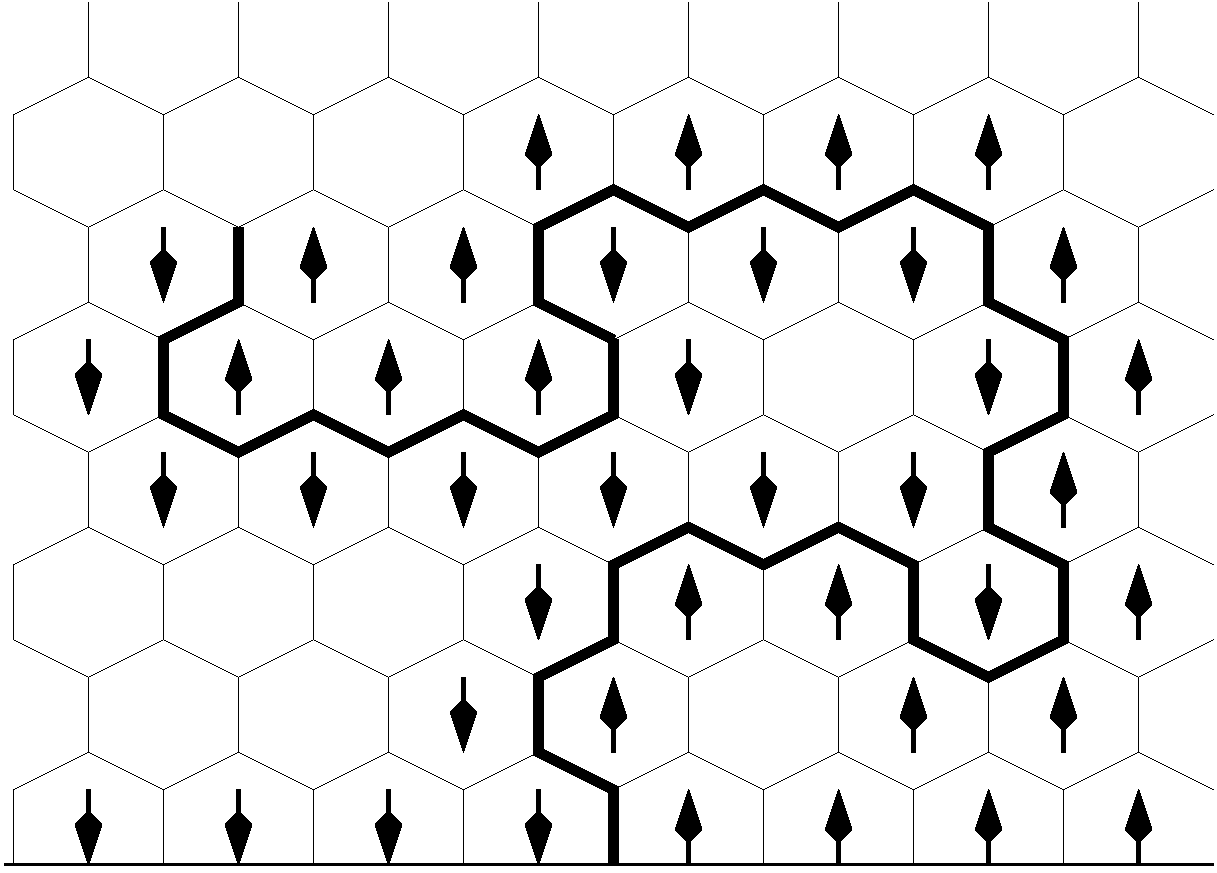
\includegraphics[height=25mm]{explore.pdf}
      \caption{SLE -- continuous limit of interfaces}
      \label{fig:sle}
      \hfill
      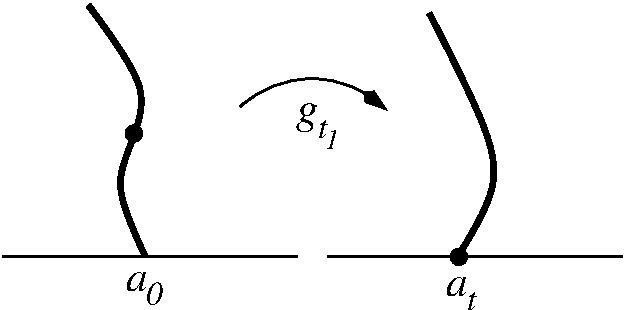
\includegraphics[width=50mm]{loewner.pdf}
      \caption{Conformal map}
      \label{fig:sle}
    \end{multicols}

  \end{figure}
\end{frame}

\begin{frame}
  \frametitle{Correspondence between SLE and minimal models of CFT}
  Consider lattice observable $\mathcal{O}$, then
  \begin{equation*}
    \prec \mathcal{O} \succ_{\mathbb{H}}=\mathbb{E}\left[\prec\mathcal{O}\succ_{\gamma_{t}}\right]=\sum_{\gamma_{t}} P\left[C_{\gamma_{t}}\right] \prec \mathcal{O} \succ_{\gamma_{t}}
  \end{equation*}
  $\prec \mathcal{O} \succ_{\mathbb{H}}$ does not depend on $t$, hence $\prec\mathcal{O}\succ_{\gamma_{t}}$ is a martingale.

  Continuous limit in critical point leads to CFT correlation function
  \begin{equation*}
    \prec \mathcal{O} \succ_{\mathbb{H}_{t}}\to \mathcal{F}(\left\{z_{i}\right\})_{\mathbb{H}_{t}}=
    \frac{\left< \mathcal{O}(\{z_{i}\})\phi(z_{t})\phi^{\dagger}(\infty)\right>_{\mathbb{H}_{t}}}{\left<\phi(z_{t})\phi^{\dagger}(\infty)\right>_{\mathbb{H}_{t}}}=
    \frac{\left< ^{g_{t}}\mathcal{O}\phi(\xi_{t})\phi^{\dagger}(\infty)\right>_{\mathbb{H}}}{\left<\phi(z_{t})\phi^{\dagger}(\infty)\right>_{\mathbb{H}}}
  \end{equation*}
  Here $\phi$ is boundary condition changing operator. 


  Or after conformal map $w(z):\mathbb{H}\setminus\gamma_{t}\to \mathbb{H}$
  \begin{equation*}
    \mathcal{F}(\left\{z_{i}\right\})_{\mathbb{H}_{t}}=\prod \left(\frac{\partial w(z_{i})}{\partial z_{i}}\right)^{h_{\lambda_i}} 
    \prod \left(\frac{\partial \bar w(\bar z_{i})}{\partial \bar z_{i}}\right)^{h_{\lambda^{*}_i}}
        \mathcal{F}(\left\{w_{i}, \bar w_{i}\right\})_{\mathbb{H}}
  \end{equation*}
  Consider evolution from $t$ to $t+dt$. First factor gives us $-\frac{2h_{\lambda_{i}}}{w_{i}^{2}}\left(\frac{\partial w_{i}}{\partial z_{i}}\right)^{h_{\lambda_{i}}}$. For fields we have 
$d\phi_{\lambda_{i}}(w_{i}) = \mathcal{G}_{i}\phi_{\lambda_{i}}(w_{i})=\left(\frac{2dt}{w_{i}}-\sqrt{\kappa} d\xi_{t}\right) \partial_{w_{i}}\phi_{\lambda_{i}}(w_{i})$
\end{frame}
\begin{frame}
  \frametitle{SLE martingales}
  We have
  \begin{equation*}
    \mathbb{E}\left[\prec\mathcal{O}\succ_{\gamma_{t}}\right]=    \mathbb{E}\left[\prec\mathcal{O}\succ_{\gamma_{t+dt}}\right], \quad \mathbb{E}\left[d \prec\mathcal{O}\succ_{\gamma_{t}}\right]=0
  \end{equation*}
  we use Ito calculus to get
  \begin{equation*}
    \left(\prod_{i=1}^{2N}\left(\frac{\partial w_{i}}{\partial z_{i}}\right)^{-h_{i}}\right)\mathbb{E}\left[d 
      \mathcal{F}_{\mathbb{H}_{t}}\right]=\left(-\sum_{i=1}^{2N}\frac{2h_{i}dt}{w_{i}^{2}}+\mathbb{E}\left[\sum_{i=1}^{2N}\mathcal{G}_{i}+\frac{1}{2}
        \sum_{i,j}\mathcal{G}_{i}\mathcal{G}_{j}\right]\right)\mathcal{F}_{\mathbb{H}}
  \end{equation*}
  Then use explicit form of conformal map and obtain
  \begin{equation*}
    \left( \sum_{i}\left[-\frac{2h_{i}}{w_{i}^{2}} +\frac{2}{w_{i}}\partial_{w_{i}}\right]+\frac{\kappa}{2}\sum_{i,j}\partial_{w_{i}} \partial_{w_{j}}\right)\mathcal{F}(\left\{z_{i}\right\})=0
  \end{equation*}

  We can rewrite it as the necessary condition on b.c.c. operator $\phi$:
  \begin{equation*}
    (L_{-2}-\frac{\kappa}{2}L_{-1}^{2})\phi=0 \Longrightarrow \phi \left|0\right>  \text{has level 2 null state}, \phi\sim \phi_{1,2} \;\text{or}\; \phi_{2,1}
  \end{equation*}

\end{frame}

\section{SLE and WZNW models}
\label{sec:sle-wzw-models}

\begin{frame}
  \frametitle{WZNW models}
  The action is written in terms of map $g:S^{2}\to G$:
  \begin{multline*}
    S=-\frac{k}{8\pi}\int d^2x\; \mathcal{K} (g^{-1}\partial^{\mu}g, g^{-1} \partial_{\mu}g)  
    \\
    - \frac{k }{24\pi^{2}} \int_{B}\epsilon_{ijk} \mathcal{K}\left(
      \tilde g^{-1}\frac{\partial \tilde g}{\partial y^i},\left[
      \tilde g^{-1}\frac{\partial \tilde g}{\partial y^j}
      \tilde g^{-1}\frac{\partial \tilde g}{\partial y^k}\right]\right) d^3y
  \end{multline*}
  \begin{itemize}
  \item   Currents 
    \begin{equation*}
      J(z)= -k \partial_zg g^{-1}\quad \bar J(\bar z)=k g^{-1}\partial_{\bar z}g
    \end{equation*}

  \item Gauge invariance
    \begin{equation*}
      g(z,\bar z)\to \Omega(z)g(z,\bar z)\bar \Omega^{-1}(\bar z),
    \end{equation*}
    where $\Omega,\;\bar \Omega \in G$

  \item Ward identities $\Omega=1+\omega$:
    \begin{equation*}
      \label{eq:87}
      \delta_{\omega,\bar \omega}\left< X \right>=-\frac{1}{2\pi i}\oint dz \sum\omega^a \left< J^a X\right>+
      \frac{1}{2\pi i} \oint d\bar z \sum \bar \omega^a \left< \bar J^a X\right>
    \end{equation*}
  \end{itemize}
\end{frame}

\begin{frame}
  \frametitle{Primary fields}
  \begin{itemize}
  \item Mode expansion gives commutation relations of affine Lie algebra $\gfh$: 
    \begin{equation*}
      \left[J^a_n,J^b_m\right]=\sum_c i f^{abc}J^c_{n+m}+kn\delta^{ab}\delta_{n+m,0} \quad \text{where} \quad           J^a(z)=\sum\limits_{n\in \mathbb Z}z^{n-1}J^a_n 
    \end{equation*}
  \item Sugawara construction $  L_n=\frac{1}{2(k+h^v)}\sum\limits_a\sum\limits_m:J^a_m J^a_{n-m}:$ -- embedding $Vir\subset U(\gfh)$.
  \item Chiral algebra $\gfh \ltimes Vir$:
    \begin{equation}
      \label{eq:92}
      \begin{aligned}
        \left[L_n,L_m\right]=(n-m)L_{n+m}+\frac{c}{12}(n^3-n)\delta_{n+m,0}\\
        \left[L_n,J^a_m\right]=-mJ^a_{n+m}
      \end{aligned}
    \end{equation}

  \item Primary fields $\phi_{\lambda}$ are labeled by highest weights of representations:
    \begin{equation*}
      \begin{aligned}
        & J_0^a\left|\phi_{\lambda}\right>=-t^a_{\lambda}\left|\phi_{\lambda}\right>  \quad    J^a_n\left|\phi_{\lambda}\right>=0 \quad \mbox{for}\; n>0 \\
        & L_0\left|\phi_{\lambda}\right>=\frac{1}{2(k+h^v)}\sum_aJ^a_0J^a_0\left|\phi_{\lambda}\right>=\frac{(\lambda,\lambda+2\rho)}{2(k+h^v)}\left|\phi_{\lambda}\right>=h_{\lambda} \left|\phi_{\lambda}\right>
      \end{aligned}
    \end{equation*}
  \end{itemize}
\end{frame}

\begin{frame}
  \frametitle{SLE and WZNW models}
  Similarly to minimal models we consider observable
  \begin{equation*}
    \mathcal{F}(\left\{z_{i}\right\})_{\mathbb{H}_{t}}=
    \frac{\left<\phi_{\Lambda}(z_{t}) \phi_{\lambda_1}(z_{1}) \dots \phi_{\lambda_n}(z_{n}) \phi_{\lambda^{*}_1}(\bar z_{1}) \dots \phi_{\lambda^{*}_n}(\bar z_{n})
        \phi_{\Lambda^{*}}(\infty)\right>}{\left<\phi_{\Lambda}(z_{t})\phi_{\Lambda^{*}}(\infty)\right>}
  \end{equation*}
  Or after conformal map $w(z):\mathbb{H}\setminus\gamma_{t}\to \mathbb{H}$
  \begin{equation*}
    \mathcal{F}(\left\{z_{i}\right\})_{\mathbb{H}_{t}}=\prod \left(\frac{\partial w(z_{i})}{\partial z_{i}}\right)^{h_{\lambda_i}} 
    \prod \left(\frac{\partial \bar w(\bar z_{i})}{\partial \bar z_{i}}\right)^{h_{\lambda^{*}_i}}
        \mathcal{F}(\left\{w_{i}, \bar w_{i}\right\})_{\mathbb{H}}
  \end{equation*}
  Consider evolution from $t$ to $t+dt$. First factor gives us $-\frac{2h_{\lambda_{i}}}{w_{i}^{2}}\left(\frac{\partial w_{i}}{\partial z_{i}}\right)^{h_{\lambda_{i}}}$. For fields we have
  \begin{equation*}
    d\phi_{\lambda_{i}}(w_{i}) = \mathcal{G}_{i}\phi_{\lambda_{i}}(w_{i})
  \end{equation*}
  But now we need to add random motion in $G$ to stochastic evolution:
  \begin{equation*}
    \mathcal{G}_{i}=\left(\frac{2dt}{w_{i}}-\sqrt{\kappa} d\xi_{t}\right) \partial_{w_{i}}+\frac{\sqrt{\tau}}{w_{i}}\sum_{a=1}^{\mathrm{dim} \gf}\left(d \theta ^{a} t^{a}_{i}\right)
  \end{equation*}
\end{frame}
\begin{frame}
  \frametitle{SLE martingales in WZNW models}
  Now for martingales we have
  \begin{equation*}
    \left(-2 \mathcal{L}_{-2}+\frac{1}{2}\kappa \mathcal{L}_{-1}^{2}+\frac{1}{2}\tau\sum_{a} \mathcal{J}^{a}_{-1} \mathcal{J}^{a}_{-1}\right)        \mathcal{F}(\left\{w_{i}, \bar w_{i}\right\})_{\mathbb{H}}=0
  \end{equation*}
  \begin{equation*}
    \mathcal{L}_{-n}=\sum_{i}\left(\frac{(n-1)h_{\lambda_{i}}}{(w_{i}-z)^{n}}-\frac{1}{(w_{i}-z)^{n-1}}\partial_{w_{i}}\right);\quad \mathcal{J}^{a}_{{-n}}=-\sum_{i}\frac{t^{a}_{i}}{(w_{i}-z)^{n}}
  \end{equation*}
  so 
  \begin{equation*}
\left| \psi\right>=\left(-2 L_{-2}+\frac{1}{2}\kappa L_{-1}^{2}+\frac{1}{2}\tau\sum_{a} J^{a}_{-1} J^{a}_{-1}\right) \left|\phi_{\Lambda}\right>    
  \end{equation*}
 is level two null state and $J^{a}_{1} \left|\psi\right>=0, J^{a}_{2}\left|\psi\right>=0$. Then $\kappa+\tau h^{v}=4$ and it is possible to derive additional relations connecting $\kappa, \tau, k$:
 \begin{equation*}
   \kappa=\frac{2(h^{v}-2k)}{2h_{\Lambda}h^{v}-k},\quad \tau=\frac{8 h_{\Lambda}-2}{2h_{\Lambda}h^{v}-k}  \quad\text{for}\; k\neq 2h_{\Lambda}h^{v}
 \end{equation*}
 To get complete classification use Knizhnik-Zamolodchikov equations.
\end{frame}

\section{Coset models}
\label{sec:coset-models}

\begin{frame}
  \frametitle{Gauged WZNW-models and coset construction}
  Add gauge fields $A, \bar{A}$ taking values in Lie algebra $\af\subset \gf$ to the action:
  \begin{multline*}
    S(g,A)=S_{WZNW}(g)+\\
    \frac{k}{4\pi}\int d^{2}z \left(\mathcal{K}(A, g^{-1}\bar \partial g)-\mathcal{K}(\bar A, (\partial g ) g^{-1})+\mathcal{K}(A,g^{-1}\bar A g)-\mathcal{K}(A,\bar A)\right)
  \end{multline*}

  Now current is
  \begin{equation*}
    J_{(\gf,\af)}=-k\partial g g^{-1} -k g A g^{-1}
  \end{equation*}

  From Ward identities we get
  \begin{equation*}
    \left< A^{b}(z)\phi_{1}\dots \phi_{N}\right>=\frac{2}{k+2 h^{v}_{\af}}\sum_{k}\frac{\tilde{t}^{b}_{k}}{z-z_{k}}\left<\phi_{1}\dots \phi_{N}\right>
  \end{equation*}
  Remember that for WZNW current we have OPE $J_{\gf}^{a}(z)\phi_{i}(w)\sim \frac{-t^{a}_{i}\phi(w)}{z-w}$.
%%  Commutation relations for current components are preserved.

  Algebraic structure is connected with two affine Lie algebras $\gfh, \afh: \afh\subset\gfh$. 

 Virasoro generators are given by difference of Sugawara expressions:
  \begin{equation*}
    L_{n}=L_{n}^{\gf}-L_{n}^{\af}
  \end{equation*}

\end{frame}

\begin{frame}
  \frametitle{Primary fields}

  Primary fields are labeled by pairs of weights $(\mu,\nu)\in \hf_{\gfh}\oplus \hf_{\afh}$, such that branching functions $b^{\mu}_{\nu}(q)\neq 0$. But some pairs are equivalent. This equivalence is given by the action of simple currents $(J,\tilde{J})$ such that $h_{J}-h_{\tilde{J}}=0$. 

  Conformal weight of primary field
  \begin{multline}
    L_0\left|\phi_{(\mu,\nu)}\right>=\left(\frac{1}{2(k+h^v)}\sum_aJ^a_0J^a_0-\frac{1}{2(k+h_{\af}^v)}\sum_b \tilde{J}^b_0 \tilde{J}^b_0 \right)
    \left|\phi_{\lambda}\right>=\\
    \left(\frac{(\mu,\mu+2\rho)}{2(k+h^v)}-\frac{(\nu,\nu+2\rho_{\af})}{2(k+h^v)}\right)\left|\phi_{(\mu,\nu)}\right>
  \end{multline}

%%  So $G/A$-coset theory is related to $\gf\oplus \bar{\af}$-theory.

 It is possible to obtain analogues of KZ-equations:
  \begin{equation*}
    \left\{\frac{1}{2}\partial_{i} + \sum_{i\neq j}^{N}\left(\frac{t^{a}_{i}t^{a}_{j}}{k+h^{v}}-\frac{\tilde t^{b}_{i}\tilde t^{b}_{j}}{k+h^{v}_{\af}}\right)\frac{1}{z_{i}-z_{j}}\right\} \left<\phi_{1}(z_{1})\dots \phi_{N}(z_{N})\right>=0
  \end{equation*}
\end{frame}

\begin{frame}
  \frametitle{SLE on coset space}
  For  $\gf\oplus \af$ WZNW-model we can write SLE generator of primary field transformation under stochastic evolution as
  \begin{equation*}
    \mathcal{G}_{i}=\left(\frac{2dt}{w_{i}}-\sqrt{\kappa} d\xi_{t}\right) \partial_{w_{i}}+\frac{\sqrt{\tau}}{w_{i}}\left(\sum_{a=1}^{\mathrm{dim} \gf}\left(d \theta ^{a} t^{a}_{i}\right)+\sum_{b=1}^{\mathrm{dim} \af}\left(d \tilde{\theta} ^{b} \tilde{t}^{b}_{i}\right)\right)
  \end{equation*}
%%    \begin{equation*}
%%      \mathcal{G}_{i}^{L,R}=\left(\frac{2dt}{w_{i}}-\sqrt{\kappa} d\xi_{t}\right) \partial_{w_{i}}+\frac{\sqrt{\tau}}{w_{i}}\left(\sum_{a=1}^{\mathrm{dim} \gf}\left(d \theta ^{a} t^{a}_{i}\right)\pm\sum_{b=1}^{\mathrm{dim} \af}\left(d \tilde{\theta} ^{b} \tilde{t}^{b}_{i}\right)\right)
%%    \end{equation*}

and get martingale condition
  \begin{equation*}
    \left(-2 \mathcal{L}_{-2}+\frac{1}{2}\kappa \mathcal{L}_{-1}^{2}+\frac{\tau}{2}\left( \sum_{a} \mathcal{J}^{a}_{-1} \mathcal{J}^{a}_{-1}-
        \sum_{b}\tilde{\mathcal{J}}^{b}_{-1} \tilde{\mathcal{J}}^{b}_{-1}\right)\right)        \mathcal{F}_{\mathbb{H}}=0
  \end{equation*}

which can be rewritten as the requirement for
\begin{equation*}
  \psi=\left(-2L_{-2}+\frac{1}{2}\kappa L_{-1}^{2}+\frac{1}{2}\tau \left(\sum_{a=1}^{\mathrm{dim}\gf}J^{a}_{-1}J^{a}_{-1}-\sum_{b=1}^{\mathrm{dim}\af}\tilde{J}^{b}_{-1}\tilde{J}^{b}_{-1}\right)\right) \phi_{(\Lambda,\Gamma)}
\end{equation*}
to be level two null-field.
\end{frame}



\begin{frame}
  \frametitle{Parafermions}
  $\mathbb{Z}(N)$ parafermions are equivalent to $SU(2)_{N}/U(1)$ coset theory.
  
  Parafermionic field decomposes as
  \begin{equation*}
    \Phi^{j}=\phi_{j}(z) \exp\left( -i \frac{j}{\sqrt{N}}\phi(z)\right)
  \end{equation*}
  where $\phi_{j}(z)$ is field of $SU(2)$-WZNW model with spin $j$, $\phi(z)$ -- $U(1)$ bosonic field.
  
  For parafermionic current we have
  \begin{equation*}
    \Psi^{\pm}=\frac{1}{\sqrt{N}} J^{\pm}\exp\left(\mp i \frac{1}{\sqrt{N}}\phi(z)\right)
  \end{equation*}
%%  Its action in terms of primary fields of $su(2)\oplus u(1)$ WZNW-model is equivalent to $J^{\pm}\pm \tilde{J}^{\pm}$.

  Martingale condition can be rewritten as
  \begin{equation*}
    \left(-2 L_{-2}+\frac{\kappa}{2}L_{-1}^{2}+\frac{\tau}{2}\left[\Psi^{+}_{-1}\Psi^{-}_{-1}+\Psi^{-}_{-1}\Psi^{+}_{-1}\right]\right) \left|\Phi\right>=0
  \end{equation*}
  which coincides with the result of Santachiara [arXiv:0705.2749].
\end{frame}

\begin{frame}
  \frametitle{Next steps}
  \begin{itemize}
  \item Act on $  \psi=\left(-2L_{-2}+\frac{1}{2}\kappa L_{-1}^{2}+\frac{1}{2}\tau \left(\sum\limits_{a=1}^{\mathrm{dim}\gf}J^{a}_{-1}J^{a}_{-1}+\sum\limits_{b=1}^{\mathrm{dim}\af}\tilde{J}^{b}_{-1}\tilde{J}^{b}_{-1}\right)\right) \phi_{(\Lambda,\Gamma)}$ with $J^{(a,b)}_{1}, J^{(a,b)}_{2}$ and get relations connecting $\kappa, \tau, k$. 
  \item Use Knizhnik-Zamolodchikov equations to simplify them.
  \item Get conditions on boundary condition changing operator
  \item Compare these conditions with results of  the study of boundary states with fusion algebra (Verlinde formula for Cardy states)
  \end{itemize}
\end{frame}

\section{Conclusion}
\label{sec:conclusion}


\begin{frame}
  \frametitle{Conclusion}
  \begin{itemize}
  \item It is possible to match SLE observables and CFT correlators
  \item Martingale conditions are equivalent to Verma module of affine Lie algebra having singular weights at level two.
  \item Primary fields of $\gf\oplus \af$ WZNW-model with equivalence relations can be used to study coset theory
  \item Study of martingale conditions in coset theory is parallel to the study of boundary states with fusion algebra
  \end{itemize}
\end{frame}

\begin{frame}
  \frametitle{Thank you for your attention!}
\end{frame}
\end{document}
